
\documentclass{IOS-Book-Article}

\usepackage{mathptmx}
\usepackage{rotating,todonotes, xspace}
\usepackage{amssymb}
\usepackage[section]{placeins}
\usepackage{makeidx}  % allows for indexgeneration
\usepackage{algorithm}
\usepackage{algpseudocode}
\usepackage{graphicx}
\usepackage{float}
\usepackage{subcaption}
\captionsetup{compatibility=false}
\usepackage{wrapfig}
\usepackage{array}
\usepackage{multicol}
\usepackage{amsmath}
%\usepackage{times}
%\normalfont
%\usepackage[T1]{fontenc}
%\usepackage[mtplusscr,mtbold]{mathtime}
%
\begin{document}
\begin{frontmatter}              % The preamble begins here.

%\pretitle{Pretitle}
\title{Fault Tolerance and Task Clustering\\
 in Scientific Workflows}
\runningtitle{Fault Tolerant Clustering}
%\subtitle{Subtitle}

\author[A]{\fnms{Weiwei} \snm{Chen}%
\thanks{Corresponding Author: Weiwei Chen, University of Southern California, Information Sciences Institute, Marina del Rey, CA, USA; E-mail:
weiweichen@acm.org.}},
\author[A]{\fnms{Rafael Ferreira de} \snm{silva}}
and
\author[A]{\fnms{Ewa} \snm{Deelman}}

\runningauthor{W. Chen et al.}
\address[A]{University of Southern California, Information Sciences Institute, Marina del Rey, CA, USA}
%\address[B]{University of Manchester, School of Computer Science, Manchester, U.K}

\begin{abstract}
Large scale scientific workflows can be composed of many fine computational granularity tasks. Task clustering has been proven to be an effective method to reduce execution overhead and increase the computational granularity of workflow tasks executing on distributed resources. However, a job composed of multiple tasks may have a greater risk of suffering from failures than a job composed of a single task. Our theoretic analysis and simulation results demonstrate that transient failures can have a significant impact on the runtime performance of scientific workflows that use existing clustering policies that ignore failures. We propose a general task failure modeling framework to address these performance issues. We show the necessity to consider the fault tolerance in the task clustering methods.  We further propose three horizontal methods and one vertical method to improve the runtime performance of executing workflows in dynamic environments. A trace based simulation is performed and it shows that our methods improve the workflow makespan significantly for five important applications.    
\end{abstract}

\begin{keyword}
scientific workflows\sep fault tolerance\sep scheduling\sep locality\sep high availability 
\end{keyword}
\end{frontmatter}

\thispagestyle{empty}
\pagestyle{empty}

\section*{Introduction}

Failure rate as a function of system and node Schroeder 2006
In this section we view the sequence of failure events as a stochastic process and study the distribution of its inter- arrival times, i.e. the time between failures. Through- out we focus on system 20 as an illustrative example.


Scientific workflows can be composed of many fine computational granularity tasks and the runtime of these tasks may be even shorter than the system overhead, which is the period time during which miscellaneous work other than the user’s computation is performed. If the overhead is large, the workflow execution inefficient. Task clustering [2] is a technique that merges several short tasks into a single job so that the job runtime is increased and the total system overhead is decreased. However, existing clustering strategies ignore or underestimate the impact of the occurrence of failures on system behavior, despite the current and increasing importance of failures in large-scale distributed systems, such as Grids [3], Clouds [4] and dedicated clusters. Many researchers [5][12][13][14][15] have emphasized the importance of fault tolerance design and indicated that the failure rates in modern distributed systems are significant. Among all possible failures, in our work we focus on transient failures because they are expected to be more prevalent than permanent failures [5]. For example, denser integration of semiconductor circuits and lower operating voltage levels may increase the likelihood of bit-flips when circuits are bombarded by cosmic rays and other particles [5]. Based on their occurrence, we divide the transient failures into two categories: task failure and job failure. In task clustering, a clustered job consists of multiple tasks. If the transient failure occurs to the computation of a task (task failure), other tasks within the job do not necessarily fail. If the transient failure occurs to the clustered job (job failure), all of its tasks fail. Accordingly, we have two models. In the task failure model (TFM), the failure of a task is a random event that is independent of the workflow characteristics and execution environment. The task failure rate is the average occurrence rate of task failures. Similarly we can define the job failure rate as the average occurrence rate of job failures and a job failure model (JFM) in which job failure is a random event. 

In a faulty environment, there are several options for managing workflow failures. First, one can simply retry the entire job when its computation is not successful as in the Pegasus framework [7]. However, some of the tasks within the job may have completed successfully and it could be a waste of time and resources to retry all of the tasks. Second, the application process can be periodically checkpointed so that when a failure occurs, the amount of work to be retried is limited. However, the overheads of checkpointing can limit its benefits [5]. Third, tasks can be replicated to different nodes to avoid location-specific failures. However, inappropriate clustering (and replication) parameters may cause severe performance degradation if they create long-running clustered jobs. As we will show, a long-running job that consists of many tasks has a higher job failure rate even when the overall task failure rate is low.   

We propose three methods to improve the existing clustering techniques (with job retry and task replication) in a faulty environment if the transient failures satisfy the task failure model. The first solution dynamically adjusts the clustering factor according to the detected task failure rate. The second technique retries the failed tasks within a job. And the last solution is a combination of the first two approaches. We further improve our methods to be able to handle the situations where task failure rate is not fully independent of workflow characteristics or execution environment. Samak [18] et al. have analyzed 1,329 real workflow executions across six distinct applications and concluded that the type and the host id of a job are among the most significant factors that impacted failures. Task specific failure is a type of failure that only occurs to some specific types of tasks. Location specific failure only occurs to some specific execution nodes. What is more, we present two refinements to handle the situation when there are fewer jobs than available resources. 

In this paper, we assume that failures can be observed from the outputs or logs of a job. We only focus on transient failures and we assume that after a finite number of retries these jobs can be completed successfully. 

Our contributions include two models to classify transient failures. We present three methods that can improve the runtime performance of workflows when transient failures occur to the tasks in a workflow. We evaluate our methods with two workflows in a simulation-based approach. 

\section{Design and Models}

\subsection{Workflow Model}

We model workflows as Directed Acyclic Graphs (DAGs), where jobs represent users’ computation to be executed and directed edges represent data or control flow dependencies between the jobs. An unclustered job contains only one task that has one process or computation. A clustered job contains multiple tasks to be executed in a sequence or in parallel. In our models and experiments, tasks within a job are executed in a sequential order. However, the conclusions that we draw also apply to the case of parallel execution since parallelization only reduces the overall runtime in a linear scale, while our results will show that the influence of task failures are at an exponential scale. Oftentimes, once a job fails, the job will be retried with the same configurations. 


In task clustering, the clustering factor (k) is an important parameter to influence the performance. We define it as the number of tasks in a clustered job. The reason why task clustering can help improve the performance is that it can reduce the scheduling cycles that workflow tasks go through since the number of jobs has decreased. The result is a reduction in the scheduling overhead and possibly other overheads as well [17]. Additionally, in the ideal case without any failures, the clustering factor is usually equal to the number of all the parallel tasks divided by the number of available resources. Such a naïve setting assures that the number of jobs is equal to the number of resources and the workflow can utilize the resources as much as possible. However, when transient failures exist, we claim that the clustering factor should be set based on the failure rates especially the task failure rate. Intuitively speaking, if the failure rate is high, the clustered jobs may need to retry more times compared to the case without clustering. Such performance degradation will counteract the benefits of reducing scheduling overheads. 
In this paper we only discuss the horizontal clustering [2], which clusters tasks on the same horizontal level in the DAGs. Figure 1 shows a simplified Montage workflow, which has 9 levels but we mainly focus on the major three levels (mProjectPP, mDiffFit, and mBackground). There are many other clustering methods such as vertical clustering, label clustering, and so on. Our approach can be extended to apply to them as well. 

\subsection{Task Failure Model}

%For system overhead $p(X|\theta)$, we assume it follows an Weibull distribution with known shape $\kappa=0.78$. When $x>0$, the PDF of $p(x|\theta, \kappa)$ is

%\begin{equation}
%f(x|\theta, \kappa)=\frac{\kappa}{\theta} (\frac{x}{\theta})^{\kappa-1}e^{-(x/\theta)^{\kappa}}  \nonumber
%\end{equation}

In our prior work \cite{Chen2011}, we have verified that $d$ fits gamma or Weibull distribution better than the other two distributions (Exponential and Normal). Schroeder et. al. \cite{Schroeder2006} have verified the inter-arrival time of task failures fits a Weibull distribution with a shape parameter of 0.78 or a gamma distribution better than lognormal and exponential distribution. In \cite{Sun2003, Iosup2008} Weibull distribution is one of the best fit for the workflow traces they used.  Without loss of generality, we choose Weibull distribution to represent the distribution of task runtime ($t$), system overhead ($d$) and the inter-arrival times of failures ($\gamma$).  $d$ is a random variable representing the system overheads. $t$ is a random variable representing the task runtime. has indicated that system overheads follow an exponential distribution. 

In Bayesian probability theory, if the posterior distribution $p(\theta|D, a, b)$ are in the same family as the prior distribution $p(\theta|a, b)$, the prior and the posterior are then called conjugate distributions. and the prior is called a conjugate prior for the likelihood function. For example, the Inverse Gamma family is conjugate to itself (or self-conjugate) with respect to a Weibull likelihood function: if the likelihood function is Weibull, choosing a Inverse Gamma prior over the mean will ensure that the posterior distribution is also Inverse Gamma. This simplifies the estimation of parameters since we can always represent our prior knowledge in a good-fit distribution intentionally. 

The conjugate pair of Weibull distribution is Inverse Gamma distribution, which means if the prior follows an Inverse Gamma distribution with parameters (the scale parameter $a$ and the shape parameter $b$), the posterior also follows an Inverse Gamma distribution with parameters (the scale parameter $a+n$ and the shape parameter $\displaystyle b+\sum_{i=1}^n{x_i^\kappa}$). The Maximum Likelihood Estimation  (MLE \footnote{J. Aldrich. R. A. Fisher and the making of maximum likelihood 1912-1922. Statistical Science, 12(3):162–176, 1997.}) of posterior is $\displaystyle\frac{b+\displaystyle\sum_{i=1}^n{x_i^\kappa}}{a+n+1}$. It is biased since the unbiased estimation is $\displaystyle\frac{b+\displaystyle\sum_{i=1}^n{x_i^\kappa}}{a+n-1}$. 

To sum up our model, we have
After we observe data $D$, we compute the posterior distribution of $\theta$
Conjugate prior distribution. 

\begin{eqnarray}
	\displaystyle  
	p(\theta|X, a, b)&=&\frac{p(\theta|a, b)\times p(X|\theta)}{p(X|a, b)}\nonumber  \\
	&\propto&p(\theta|a, b)\times p(X|\theta)\nonumber 
\end{eqnarray}

$X$ could be $d$, $t$ or $\gamma$ 

$p(\theta|X,a, b)$ is called the posterior distribution. We are interested in its MLE. 

$p(\theta|a, b)$ is called the prior distribution. We have already known this. 

$p(X|\theta)$ is the likelihood. We only need to know its shape parameter instead of its scale parameter, which gives us much benefits. 

\begin{figure*}[!htb]
\centering
  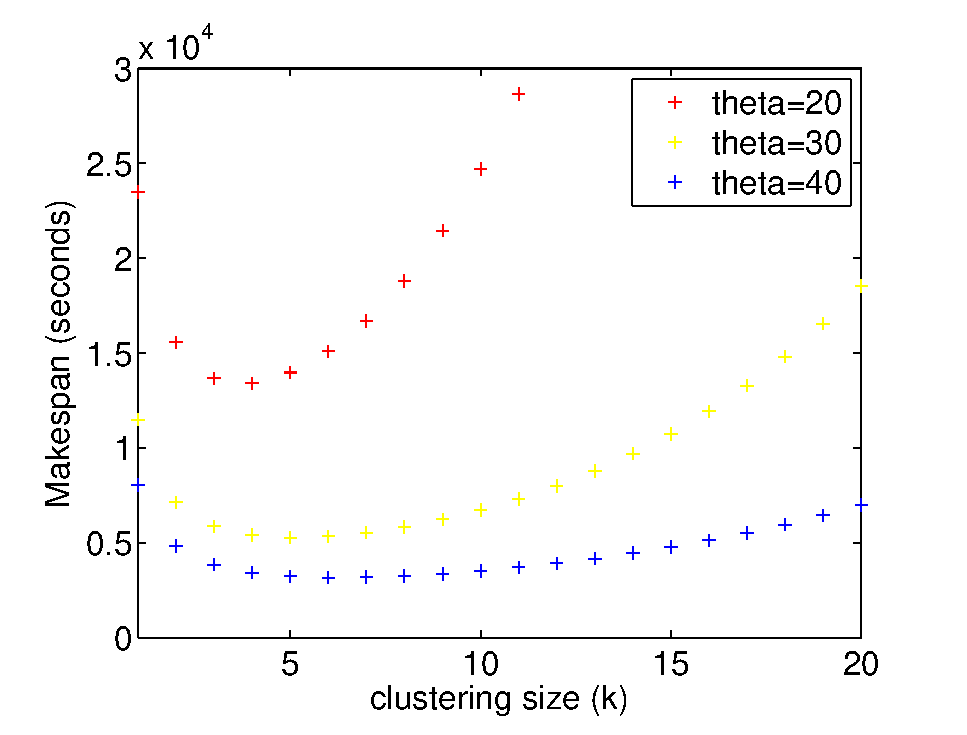
\includegraphics[width=0.95\linewidth]{figure5.eps}
  \caption{Makespan with different clustering size. (n=1000 r=20 t=5 sec, d=50 sec)}
  \label{fig:model_makespan}
\end{figure*}

\begin{figure*}[!htb]
\centering
  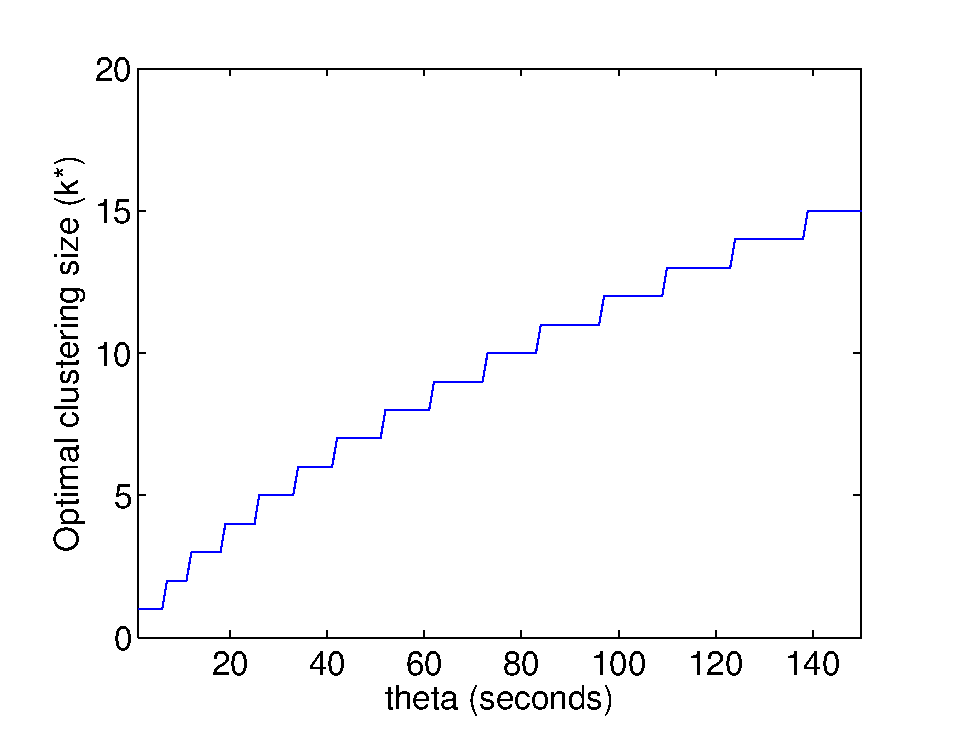
\includegraphics[width=0.95\linewidth]{figure6.eps}
  \caption{Optimal clustering size (k*) with different  theta (n=1000 r=20 t=5 sec, d=50 sec)}
  \label{fig:model_makespan}
\end{figure*}

The next step is to reduce the estimated finish time ($M$) of $n$ tasks in case the $t$, $d$ and $\gamma$ are known. $M$ includes the runtime of the clustered job and its subsequent retry jobs if the first try fails. The time to run a single task once is $t$. $k$ is the clustering size indicating the number of tasks in a clustered job. For a clustered job, let the expectation of retry times be $N$. The process to run (and retry) a job is a Bernoulli trial with only two results: success or failure. Once a job fails, it will be retried until it is eventually completed successfully because we assume the failures are transient. By definition we have, 
$\displaystyle
N=\frac{1}{1-F(kt+d)}=\frac{1}{e^{-(\displaystyle\frac{kt+d}{\theta})^{\kappa}}}
$, $F(x)$ is the CDF of $\gamma$ under known shape parameter $\kappa$ and estimated scale parameter $\theta$. 



We claim a clustered job succeeds only if all of its tasks succeed. 
We assume that $n \gg r$, but $n/k$ is not necessarily much larger than $r$ since $k$ could be very large. Normally at the beginning of workflow execution, $n/k > r$, which means there are more clustered jobs than available resources. To try all $n$ tasks once, irrespective of whether they succeed or fail, one needs approximately $\displaystyle \frac{n}{rk}$ execution cycle(s) since at each execution cycle we can execute at most $r$ jobs. Therefore, the time to execute all n tasks once is $\displaystyle\frac{n(kt+d)}{rk}$. And the time to complete them successfully in a faulty environment is $\displaystyle\frac{Nn(kt+d)}{rk} $ since each job requires $N$ retries on average.  

On the other side, at the end of the workflow execution, since n is decreasing with the process of workflow, it is possible that $\displaystyle \frac{n}{k} < r$, which means there are fewer jobs than the available resources. One needs just one execution cycle to execute these tasks once. The time to complete all $n$ tasks successfully is $N(kt+d)$. 

In summary, the estimated makespan is, 

\begin{equation} 
\label{eq:jfm}
M=
\begin{cases}
\cfrac{n(kt+d)}{rk}{e^{-(\cfrac{kt+d}{\theta})^{\kappa}}}, & \text{if } \cfrac{n}{k}\geq r \\
(kt+d){e^{-(\cfrac{kt+d}{\theta})^{\kappa}}}, & \text{else}
\end{cases}
\end{equation}
Let $k^*$ is the optimal clustering factor and $M^*$ is the minimal runtime of these $n$ tasks.  Fig.~\ref{fig:model_makespan} shows the three examples of $M$ using a low task failure rate ($\theta=40$s), a medium task failure rate ($\theta=30$s) and a high task failure rate ($\theta=20$s). Other parameters are $n=1000$, $t=5$ sec, $d=50$ sec, and $r=20$. These parameters are close to the level of mProjectPP in the Montage workflow that we simulate in Section IV. It is difficult to find a analytical solution of $k^*$. However, $k$ can only be integers in practice, which simplifies the searching process for $k^*$. 
We performed a parameter searching study, where we first estimate the upper bound of $k$ as $\displaystyle\frac{n}{r}$, and the lower bound of $k$ as 1 for simplicity. Data points are divided into ten chunks and then we sample one data point from each chunk. We then select the chunk that has the lowest makespan and set the new upper and lower bounds as the borders of the selected chunk, respectively. These steps are repeated until the upper and lower bounds have converged into a data point. 

But it has some : 1. it has one global minimal, 2. it is continuous. Thus we could use such as Newton's method to get the optimal $k^*$ and the minimal $M$. 

Even though there are multiple local minimal makespan values, these data points are close to each other, and the difference between their values (on the order of seconds) is negligible.

And then we verify our claim with a real case. 

%Need matlab simulation to get the optimal k

%Figure 2 shows the relationship between the expected runtime ttotal* and the clustering factor k in Eq. (1). We can see that the optimal clustering factor (in this example it is 50) does not change with different job failure rates. In comparison with TFM in Figure 3, the optimal clustering factor (in this example it is 5) is not equal to n/r. This conclusion is consistent with our previous claim since a clustered job has a higher chance to fail when the task failure rate is higher.

%Figure 4 shows the relationship between the task failure rate and the optimal clustering factor as indicated in Eq. (4). We can see that when the task failure rate is high (α>0.03), it is better to use no clustering at all (k<2).  We can also see that the optimal clustering factor k* decreases with the increase in the task failure rate. 
%Below we discuss to determine which model a faulty environment follows if there is no knowledge about the cause of failures (transient or permanent, task or job). By analyzing the relationship between expected runtime and clustering factor we can tell whether it tends to be TFM or JFM.  There are two criteria: 1) whether the execution runtime has an exponential increase (TFM) or linear increase (JFM) when k is large enough; 2) whether the optimal clustering factor is influenced by the failure rates (If yes, TFM; otherwise JFM).
%Also, we assume that the jobs in this workflow and the resources are homogeneous. In section IV.E and section IV.F, we extend this model to consider task specific failures and location specific failures. The job-scheduling algorithm is First-Come-First-Serve, while one may use more complex algorithms such as HEFT [9] or Min-Min [8].. 
%From this theoretic analysis, we conclude that 1) the lower the task failure rate is, the better runtime performance the task clustering has; 2) in TFM, adjusting the clustering factor according to the detected task failure rate can improve the runtime performance; 3) in JFM, we just need to set k=n/r. For the rest of our paper, we will only focus on the TFM.


\section{Fault Tolerant Clustering}

As indicated in Section II, inappropriate clustering may increase the makespan of a workflow. To improve the fault tolerance from the point of view of clustering, we propose three methods: Dynamic Clustering (DC), Selective Reclustering (SR) and Dynamic Reclustering (DR).

A.	Dynamic Clustering (DC)

Dynamic Clustering adjusts the clustering factor according to the task failure rates measured from jobs that have already been completed, either successfully or failed. Currently we use the average value of task failure records. 
 
Failure records contain the information about the number of failed tasks, the type of tasks, the resource id, and a timestamp. The type of tasks is used to detect the task specific failures and the resource id is used to detect location specific failures. Then we calculate the average task failure rate and the average job failure rate. Figure 5 shows an example where the initial clustering factor is 4 and thereby there are four tasks in a clustered job at the beginning. During execution, three out of these tasks fail. TFM suggests an optimal clustering factor to be 2, then this job will be split into two clustered jobs while each has two tasks and the two clustered jobs are then submitted for retry.  DC is not aware that there are only three failed tasks. 

According to Eq. (4), an estimation of the minimal makespan in DC can be simplified as:
                                             (5)
B.	Selective Reclustering (SR)
In DC, one knows the average task failure rate but the information about which tasks have failed is not available. In practice, it may be hard to identify the failed tasks, but if it is supported, we can further improve the performance with Selective Reclustering that selects the failed tasks in a clustered job and clusters them into a new clustered job, or treats them individually. SR is different to the naïve job retry in that the latter method retries all tasks of a failed job even though some of the tasks have succeeded. SR requires collecting the task ids in failure records. 
Figure 6 shows an example of SR. At the beginning, there are four tasks and three of them have failed. One task succeeds and exits. Only the three failed tasks are merged again into a new clustered job and the job is retried. This approach does not intend to adjust the clustering factor, although the clustering factor will be smaller and smaller naturally after each retry since there are less and less tasks in a clustered job. In this case, the clustering factor has reduced from 4 to 3.
 
Figure 6	Selective Reclustering.
C.	Dynamic Reclustering (DR)
Selective Reclustering does not analyze the failure rate rather, it uses a natural way to reduce the clustering factor if the failure rate is too high. However, it requires a special ability to select the failed tasks, while DC does not. We then propose the third method, Dynamic Reclustering, which is a combination of SR and DC to see whether using both strategies can improve workflow performance. In DR, only failed tasks are merged into new clustered jobs and the clustering factor is also adjusted according to the detected task failure rates.
 
Figure 7	Dynamic Reclustering
Figure 7 shows the steps of DR. At the last scheduling cycle, three tasks within a clustered job have failed. Therefore we have only three tasks to retry and further we need to adjust the clustering factor (in this case it is 2) according to the task failure rate. 

\section{Experiments and Discussions}

In this section, we evaluate our methods with two workflows, whose runtime information is gathered from a real execution traces. The simulation-based approach allows us to control system parameters such as task failure rate in a continuous way so as to clearly demonstrate the performance of the algorithms. Our methods can also be applied to real workflow management systems as long as they support failure logging. 

\subsection{Experiments Setup and Workflows Used}
We use a real trace of the Montage workflow [1] and the Periodogram application to evaluate our models and optimization methods. The reason why we chose Montage and Periodogram is that they represent two different types of workflows. As shown in Figure 1, Montage has complex data dependencies between tasks/jobs while Periodogram is simply a bag-of-tasks. Montage is an astronomy application used to construct large image mosaics of the sky.  Runtime data are collected from real runs under the Pegasus Workflow Management System (WMS) [7]. We ran the Montage workflow with a size of 8 degree squares of sky. The workflow has 10,422 tasks and 57GB of overall data. The workflow was run on a cluster with 20 nodes. The Periodogram application is also developed by IPAC (Caltech) to identify periodic signals from light curves that arise from transiting planets and stellar variability. The Periodogram workflow we ran has ~216,600 tasks and 19GB input data. The Periodogram workflow has only one level of tasks. 
With these runtime information and file size, we use CloudSim [6] to simulate the workflows in a controlled environment.  CloudSim is a framework for modeling and simulation of cloud computing infrastructures and services. Internally, workflow execution is divided into four steps: first, the workflow engine releases tasks based on the dependencies between tasks; second, the clustering engine merges the released tasks into jobs; third, these jobs are submitted to the job scheduler and are matched with resources based on different criteria specified by users; fourth, each job is executed by a worker node that has input files and executable files available. Each workflow was simulated at least 100 times to assure that standard deviation in the workflow makespan is less than 10%. 
To make the simulation consistent with the real results in Pegasus WMS, we modified CloudSim to execute our simulations.  Figure 8 shows the system overview of our simulation. The Workflow Engine manages tasks and jobs based on their dependencies between jobs to assure that a job may only be released when all of its parent jobs have completed successfully. It also loads workflow logs that are gathered and reconstructed from prior runs. The Clustering Engine merges tasks on the same horizontal level into clustered jobs according to the suggested clustering factor (k*). The Job Scheduler is revised to match jobs to the most reliable worker nodes and avoid or even skip a worker node that has too many failures compared to others. The Failure Generator is added to generate task failures according to the specified average task failure rate. The Failure Monitor serves as an agent that suggests clustering factor based on the estimation of the task failure rate, the type of task, and the node to be matched. Based on this information, the Clustering Engine will adjust the clustering factor in DC or DR approaches.
 
Figure 8	 System Overview
\subsection{Dynamic Performance}
To evaluate the performance of TFM and DC, we first simulated the Montage workflow with a fixed task failure rate (α = 0.002).  
 
Figure 9	Clustering Factor
Figure 9 shows the difference between the actual clustering factor and the suggested clustering factor at each scheduling interval. The scheduling cycle is a period when the Workflow Engine releases tasks that are ready to run and the Clustering Engine merges these tasks along with tasks that have failed. Montage has three major horizontal levels of tasks that require clustering, which are mProjectPP, mDiffFit, and mBackground. At the beginning, the Failure Monitor does not have enough failure records to identify the task failure rate. We adopt a risky strategy in that the initial clustering factor is set to be n/r so that all tasks will be tried once at the beginning. That is why the actual clustering factor at cycle 1 is approximately 25 and then it falls down quickly. After passing 5, the actual k and the suggested k overlap with each other since the Failure Monitor has collected enough data to adapt to the faulty environment. From the cycle 4 to 14, the workflow is mainly executing mDiffFit, and during that time the suggested k and actual k fall down to 6 eventually since our model requires some time to run jobs first and then predict the task failure rate. The suggested k and the actual k for mBackground fall to 3 quickly since at this step the prediction of task failure rate is already stabilized. The reason that each type of task has different clustering factors is that they have different runtime on average. 
  Figure 9 also reminds us that the actual k is sometimes smaller than the suggested k, which has been explained in cycle 1 to 3. At cycle 3, the actual k is smaller than the suggested k because the Clustering Engine does not have sufficient tasks to be clustered since most tasks are completed. We will address this issue and improve the performance in Section IV.D. 

\subsection{Performance of different Optimization Methods}
TABLE I	WORKFLOW MAKESPAN (MONTAGE, UNIT: SECOND) 
α	Optimization Methods
	NOOP	DC	SR	DR
0.002	9827	9010	8168	8633
0.004	11390	9224	8174	8687
0.006	13625	9430	8181	8771
0.008	16989	9590	8191	8818
0.01	22026	9709	8202	8856
0.02	169075	10218	8242	8930
0.04	44099753	10853	8316	9153
0.06	N/A 	11488	8387	9344
0.08	N/A	11951	8461	9734
TABLE II	WORKFLOW MAKESPAN (PERIODOGRAM, UNIT: SECOND) 
α	Optimization Methods
	NOOP	DC	SR	DR
0.002	17180	15141	13824	15052
0.004	18197	15272	13853	15106
0.006	18930	15360	13883	15130
0.008	19344	15464	13911	15159
0.01	19668	15566	13941	15176
0.02	19889	16081	14086	15363
0.04	21407	17141	14376	15712
0.06	24147	18283	14681	16109
0.08	26597	19511	15010	16478
We compare the workflow makespan when running the workflow with DC, SR, DR and No Optimization (NOOP) with task failure rate in a range between 0.2% and 8%. Researchers [14] show that a transient failure rate is not usually more than 10%; otherwise such a system does not have much practical usage. If the task failure rate is lower than 0.1%, one doe not need to apply our methods. 

 
Figure 10	Workflow Makespan (Periodogram)
We present the workflow makespan improvement of Montage in TABLE I and the results of Periodogram in TABLE II and Figure 10. Both improvements are significant particularly with SR since it is able to identify the failed tasks. Even though DC has optimized the clustering factor according to a prediction of task failure rate, the jobs to be retried still contain both failed tasks and successful tasks. DR performs better than DC as we have expected. Both SR and DR exclude the successful tasks and only retry the failed tasks within a job. However, they require the ability to identify tasks that have failed in a clustered job, which DC does not. These tables also show that the improvement is more significant when the task failure rate is higher, which is consistent to our previous claim. Particularly for Montage, we reduce the growth of makespan from a near-exponential increase (in NOOP) to a near-linear increase, which is a giant leap for task clustering. What is more, SR performs better than DR in the two workflows, which shows that there is still a gap between dynamically adjusting the clustering factor based on task failure rate and naturally retrying failed tasks. This might be caused by the simplification of our models and it suggests us to investigate the performance issues further.

\section{Refinements to Dynamic Clustering}
As indicated in last section, the actual clustering factor is not consistent with the suggested clustering factor in some particular cases and n >> r may not hold. When the workflow is almost done and there are not sufficient tasks available, our simplification of model may no longer be effective. To solve this problem, we propose three methods. 
The Default method tries to follow the clustering factor strictly.  . When there are insufficient tasks, they are clustered into less number of jobs than the available resources ( ). 
The Replicative method tries to follow the clustering factor too ( ) but it replicates the jobs so as to utilize idle resources ( ) by  .
The Even method tries to adjust the clustering factor ( ) so as the number of jobs is equal to the number of resources ( ).  The resource utilization is improved too. 
Figure 11 shows the performance of three refinements with the Montage workflow. We can see that the Replicative method can reduce the runtime by up to 19% compared to the Default method while the Even method does not improve the performance much. The reason is that adjusting the clustering factor would cause performance degradation although resource utilization is improved. 
 
Figure 11	Performance of different refinements (Montage)
\subsection{Task Specific Failures}
TABLE III	PERFORMANCE WITH TASK SPECIFIC FAILURE DETECTION (MONTAGE, UNIT:SECOND). 
α 	Optimization Methods
	DR	DR+TSFD	DC	DC+TSFD
0.2	10415	10412	13804	13820
0.4	11830	11839	22946	22923
0.6	14704	14688	60429	60414
0.8	23238	23229	436638	435297
In this section, we improve DR and DC with Task Specific Failure Detection (TSFD). The Failure Monitor module regularly collects failure records including the task id of the failed task and then calculates the task failure rate per task type. The Clustering Engine then adjusts the clustering factors based on different task failure rates. In this experiment, we set the task failure rate of mProjectPP and mDiffFit to be 0.001 while the task failure rate of mBackground ranges from 0.2 to 0.8. TABLE III shows the performance of DC+TSFD and DR+TSFD. Neither of them show significant improvement. The reason is that Montage has almost the same number (~2,000) of mProjectPP, mDiffFit and mBackground jobs. Therefore, the estimated task failure rate of mBackground is one third of its real task failure rate. Figure 3 tells that TFM is relatively robust to the change of task failure rate when the clustering factor is small. This conclusion also suggests that the estimation of task failure rate does not have to be very precise. 

\subsection{Location Specific Failures }
In this section, we improve DC, SR and DR with Location Specific Failure Detection (LSFD).  The Failure Monitor remembers the resource id (worker node) where the failure has occurred and calculates the task failure rates for each worker node. The Job Scheduler then tries to avoid unstable worker nodes or even skip them if the task failure rates are higher than a threshold. Figure 12 shows an example when two out of twenty nodes have a higher task failure rates (from 0.2 to 0.8) while others still have a task failure rate of 0.001. We can see that the DC+LSFD has significant improvement of up to 62% while SR+LSFD and DR+LSFD do not have much improvement. The reason of the spike (DC without LSFD) is that it detects many failures and then creates many small jobs, which increases the impact of scheduling overhead and other possible overheads. 
 
Figure 12	Performance with location specific failure detection (Montage).   
\section{RELATED WORK}
Failure analysis and modeling [12] presents system characteristics such as error and failure distribution and hazard rates. Schroeder et al. [13] has studied the statistics of the data, including the root cause of failures, the mean time between failures, and the mean time to repair. Sahoo et al. [14] analyzed the empirical and statistical properties of system errors and failures from a network of heterogeneous servers running a diverse workload. Oppenheimer et al. [15] analyzed the causes of failures from three large-scale Internet services and the effectiveness of various techniques for preventing and mitigating service failure. McConnel [16] analyzed the transient errors in computer systems and showed that transient errors follow a Weibull distribution. Benoit [19] et al. analyzed the impact of transient and fail-stop failures on the complexity of task graph scheduling. Based on these work, we measure the failure rates in a workflow and then provide methods to improve task clustering.  
Task clustering [2] merges fined-grained tasks into coarse-grained jobs. After task clustering the number of jobs is reduced and the cumulative overhead is reduced too. However, their clustering strategy is static and does not consider the dynamic resource characteristics. In addition, we discover that inappropriate clustering parameters would damage the benefits of task clustering. Also, they did not consider the middleware overhead that relates to the overhead of grid middleware services, such as the time to query resources, the time to match jobs with resources, etc. These overheads are included in our model in the form of constant delays and the values are set based on real traces. 
Dynamic job grouping is a technique that dynamically assembles the individual fined-grained tasks into a group of jobs and send these coarse-grained jobs to the resources.  Muthuvelu [11] et al. has taken into account the characteristics of jobs and the costs of resources. Liu [10] et al. extended the work to consider the dynamic resource characteristics and the processing capability and bandwidth to constrain the sizes of coarse-grained jobs. Compared to their work, our work focuses on the failure occurrence and aims to improve the makespan of a workflow in a faulty environment. 

\section{Future Work}

In the future, we plan to apply our work to a real world framework---the Pegasus Workflow Management System and to evaluate the performance with more applications. We will also examine failures with different distribution, such as for example Weibull.  We will further evaluate the robustness of our methods to the variance of failure patterns, runtime, and overhead. The gap between DC and SR indicates that there is still space for further improvement in the approach of dynamically adjusting the workflow task clustering factor. 

\section{ACKNOWLEDGMENT}
This work is supported by NFS under grant number IIS-0905032. We thank Gideon Juve, Karan Vahi, Mats Rynge and Rajiv, Mayani for their help. 


\bibliographystyle{elsarticle-num}
\bibliography{biblio}

\end{document}
